\documentclass[tikz,border=8pt]{standalone}

\usepackage{fontspec}
\setmonofont{Hack}

\usetikzlibrary{arrows.meta,positioning}

\begin{document}
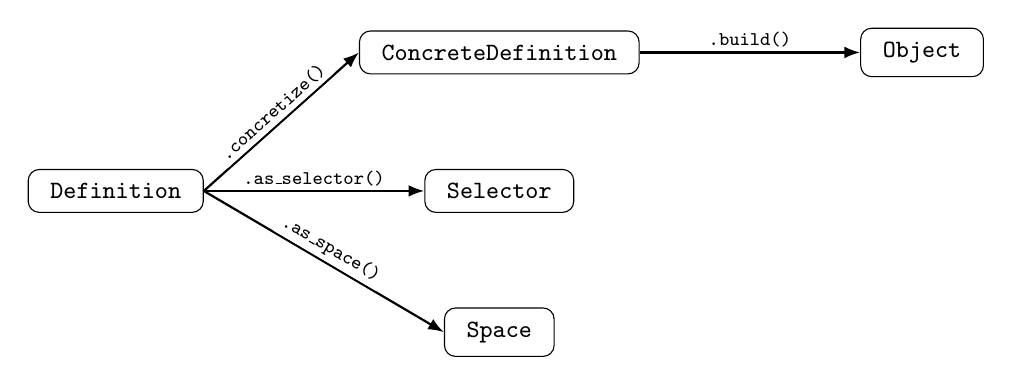
\begin{tikzpicture}[
  node distance=12mm and 28mm,
  entity/.style={
    draw,
    rounded corners,
    inner xsep=8pt,
    inner ysep=5pt,
    align=center,
    font=\small
  },
  relation/.style={
    -{Latex[length=2mm]},
    thick
  },
  edge label/.style={
    midway,
    fill=white,
    inner sep=1.5pt,
    font=\scriptsize
  }
]

% Nodes
\node[entity] (d) {\texttt{Definition}};
\node[entity, right=of d] (sl) {\texttt{Selector}};
\node[entity, above=of sl] (cd) {\texttt{ConcreteDefinition}};
\node[entity, below=of sl] (sp) {\texttt{Space}};
\node[entity, right=of cd] (o) {\texttt{Object}};

% Relationships
\draw[relation] (d.east) -- node[edge label, above, sloped] {\texttt{.concretize()}} (cd.west);
\draw[relation] (d.east) -- node[edge label, above, sloped] {\texttt{.as\_selector()}} (sl.west);
\draw[relation] (d.east) -- node[edge label, above, sloped] {\texttt{.as\_space()}} (sp.west);
\draw[relation] (cd.east) -- node[edge label, above, sloped] {\texttt{.build()}} (o.west);

\end{tikzpicture}
\end{document}
